\documentclass{article}
\usepackage{graphicx} % Required for inserting images
\usepackage[margin=2cm]{geometry} 
\usepackage{multicol,amsmath, amssymb}
\usepackage{xcolor}


\begin{document}
\begin{center}
    {\LARGE \textbf{Probability} }
\end{center}

\begin{multicols}{2}

\begin{itemize}

    \item An experiment is said to be a \textbf{random experiment} if there is more than one possible outcome, and it is impossible to predict the outcome in advance.An experiment is said to be a random experiment if there is more than one possible outcome, and it is impossible to predict the outcome in advance.
    \item All possible results of an experiment are called its \textbf{outcomes}.
    \item Set of all these outcomes is known as the \textbf{sample space} and is denoted by ‘S’.
     \item Any subset E of a sample space S is called an \textbf{event}.
     
    \item the event E of a sample space S is said to have \textbf{occurred} if the outcome of the experiment is such that  $\omega \in  E$. If the outcome $\omega$ is such that $\omega \not \in E$, we say that the event E has \textbf{not occurred}.

    \subsection*{\large \textcolor{red}{Types of events}}
    \begin{enumerate}
        \item  \textbf{Impossible event and sure event}:The empty set $\phi$ and the sample space S describe the impossible event and sure event respectively.
        \item \textbf{Simple event} : An event E having only one sample point of a sample space.
        \item  \textbf{Compound event}: An event having more than one sample point of a sample space.
    \end{enumerate}

    \textbf{Example}: 

    Consider the experiment of rolling a die. The associated sample space is
   $$ S = \{1, 2, 3, 4, 5, 6\}$$
   \begin{itemize}
       \item The event “ the number appears on the die is a multiple of 7” is impossible (E=$\phi$)
       \item The Event “the number turns up is odd or even” is sure ( $ E = \{1, 2, 3, 4, 5, 6\}$)
       \item The Event“ the number appears on the die is an odd prime” is simple(E=\{2\})
       \item The Event“ the number appears on the die is even" is compound (E=\{2,4,6\})
   \end{itemize}
\end{itemize}

\subsection*{\large \textcolor{red}{Algebra of events}}
Let A, B, C be events associated with an experiment whose sample space is S.Then 
\begin{enumerate}
    \item     Event ‘not A’ = $A’$
    \item Event ‘A or B’ = $A \cup B$
    \item Event ‘A and B’ = $A \cap B$
    \item Event ‘A but not B’ = A – B =$A \cap B'$
    \item Event 'Neither A nor B' ='not A and not B' =$A' \cap B'$=$(A \cup B)'$
\end{enumerate}

Let $A,B,E_1,E_2,\dots , E_n$ are events of an experiment .Then
\begin{itemize}
    \item If $A \cap B = \phi$, then A and B are mutually exclusive events or disjoint events.
    \item If $E_1 \cup E_2 \cup E_3 \cup \dots \cup E_n = S$, then we say that $E_1, E_2, E_3, \dots, E_n$ are exhaustive events.
    \item If $E_1 \cup E_2 \cup E_3 \cup \dots \cup E_n = S$, and $E_i \cap E_j = \phi$, $i \not = j$ then we say that $E_1, E_2, E_3, \dots, E_n$ are mutually exclusive events and exhaustive events.

    
\end{itemize}

\subsection*{\large \textcolor{red}{Axiomatic Approach to Probability}}
Let S be the sample space of a random experiment. The probability P is a real
valued function whose domain is the power set of S and range is the interval [0,1]
satisfying the following axioms
\begin{enumerate}
    \item[(i)] For any event E, $P (E) \geq 0$
    \item[(ii)]P(S) = 1
    \item[(iii)] If E and F are mutually exclusive events, then P($E \cup F$) = P(E) + P(F). 
\end{enumerate} 

Let S be a sample space containing outcomes $\omega_1 , \omega_2 ,\dots, \omega_n$ , i.e.,
$S = \{\omega_1, \omega2, \dots, \omega_n\}$
It follows from the axiomatic definition of probability that\\
(i) $0 \leq P (\omega_i) \leq 1$ for each $\omega_i \in S$\\
(ii) $P (\omega_1) + P (\omega_2) + \dots + P (\omega_n) = 1$\\
(iii) For any event A, $P(A) = \Sigma P(\omega_i )$, $\omega_i \in A$.


\subsection*{\large \textcolor{red}{Probability of an event}}
Let S is a sample space and E be an event, such that n(S) = n and n(E) = m. If each outcome is equally likely, then it follows that $P(E) = \frac{m}{n}$.

\begin{enumerate}
    \item If A and B are any two events, then $P(A \cup B) = P(A) + P(B) – P(A \cap B)$
    \item If A and B are mutually exclusive events, then $P(A \cup B) = P(A) + P(B)$ , $P(A \cap B)=\phi$
    \item If A is any events, then P(A$’$) = 1 – P(A)
\end{enumerate}

\end{multicols}
\pagebreak

\begin{center}
    {\LARGE \textbf{Permutations and Combinations} }
\end{center}

\begin{multicols}{2}

\subsection*{\textcolor{red}{Fundamental Principle of Counting}}
If an event can occur in ‘m’ different ways, following which another event can occur in ‘n’ different ways, then the total number of occurrences of the events in the given order is m × n.

\textbf{Example }:
Mohan has 3 pants and 2 shirts.Then there are $3 \times 2=6 $ pairs of pant and shirt

\subsection*{\large \textbf{\textcolor{red}{Permutation}}}
A permutation is the arrangement of some or all of a number of different objects.

\subsubsection*{Factorial notation}
The notation n! represents the product of first n natural numbers,


   \begin{align*}
   n!&=1.2.3\dots n\\
     &=n(n-1)!\\
    &=n(n-1)(n-2)!\\
    &=n(n-1)(n-2)(n-3)!   
    \end{align*} 
    
\begin{itemize}

    \item 1!=1
    \item 0!=1
\end{itemize}

\subsection*{Theorem}
The number of permutation of ‘n’ different objects taken ‘r’ at a time, where the objects do not repeat is n(n – 1)(n – 2)……(n – r + 1) which is denoted by $^nP_r$
\begin{itemize}
    \item $^nP_r=\frac{n!}{(n-r)!},0<r\leq n$ 
    \item $^nP_n=n!$
    \item $^nP_0=1$
    \item $^nP_1=n$
\end{itemize}

\subsection*{Theorem}
The number of permutations of n different objects taken r at a time,
where repetition is allowed, is $n^r$.
\subsection*{Permutation when all the objects are not distinct.}
\begin{enumerate}
    \item The number of permutations of ‘n’ objects, where ‘p’ objects are of the same kind and rest all different = $\frac{n!}{p!}$
    \item  The number of permutations of ‘n’ objects, where ‘$p_1$’ objects are of one kind, ‘$p_2$’ objects are of the second kind, …….., ‘$p_k$‘ objects are of a $k^{th}$ kind and rest all different =$\frac{n!}{p_1! \times p_2! \times \dots p_k!}$
\end{enumerate}

\subsection*{\textcolor{red}{Combinations}}
A combination is a selection of some or all of a number of different objects (the order of selection is not important). The number of selection of ‘n’ things taken ‘r’ at a time is $^nC_r=\frac{n!}{(n-r)!r!}$

\begin{itemize}
    \item $^nP_r=^nC_r .r!$
    \item $^nC_r=\frac{n!}{(n-r)!}, 0 <r \lq n $ 
    \item $^nC_n=^nC_0=1$
    \item $^nC_1=1$
    \item $^nC_r=^nC_{n-r}$
    \item $^nC_r+^nC_{r-1}=^{(n+1)}C_r$
\end{itemize}

\end{multicols}











\begin{center}
    {\LARGE \textbf{Binomial Theorem} }
\end{center}

\begin{multicols}{2}
The expansion of a binomial for any positive integral ‘n’ is given by
$$(a+b)^n=^nC_0 a^n+ ^nC_1 a^{n-1}b+^nC_2 a^{n-2}b^2+\dots + ^nC_n b^n$$

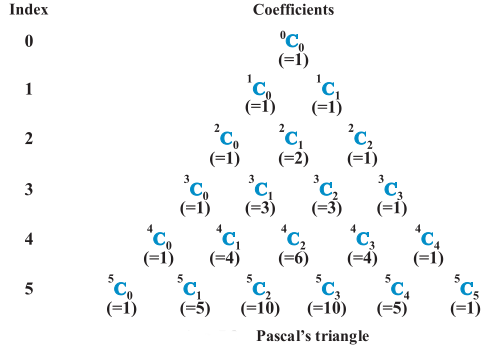
\includegraphics[scale=0.5]{1.png}




\subsection*{\large \textcolor{red}{Observations}}
\begin{itemize}
    \item The notation $\Sigma_{k=0}^n {^nC_k} a^k b^{n-k}$  stands for $^nC_0 a^n+ ^nC_1 a^{n-1}b+^nC_2 a^{n-2}b^2+\dots + ^nC_n b^n$
    \item The general term in the expansion is $t_{r+1} = ^nC_r a^{n-r} b^r$
    \item The coefficients $^nC_r$ occuring in the binomial theorem are known as binomial
    \item There are (n+1) terms in the expansion of ($a+b)^n$, i.e., one more than the index
coefficients.
\item Middle term in the expansion is $\left(\frac{n}{2}+1\right)^{t h}$ term if n is even , $\left(\frac{n+1}{2}\right)^{t h}$ and $\left(\frac{n+1}{2}+1\right)^{b_{t}}$ term if n is odd 
\end{itemize}


\end{multicols}










\end{document}
